\begingroup
\renewcommand*{\arraystretch}{1.5}
\begin{table}[b]
	\centering
	\begin{tabular}{c | c | c | c}
		\multirow{2}{*}{$ w_0 $ [$ \mu\mathrm{m} $]} & \multicolumn{3}{c}{Total absorption of laser energy [\%]} \\ \cline{2-4}
		 & const. $ E = 2.83 \cdot 10^{4} \ \mathrm{J} $ & const. $ I = 10^{20} \ \mathrm{W/cm^2} $ & const. $ I = 10^{21} \ \mathrm{W/cm^2} $ \\ \hline \hline
		0.5 & 20.12 & 16.23 & 31.77 \\ \hline
		1.0 & 9.59 & 9.59 & 23.76 \\ \hline
		2.0 & 5.27 & 8.26 & 23.82 \\ \hline
		4.0 & 3.49 & 8.29 & 23.71 \\
	\end{tabular}
	\caption{A summary of the rates of the total laser energy absorption in plasma for several different sizes of the focal spot and different laser intensities.}
	\label{table:2}
\end{table}
\endgroup

In this section, the results of simulations performed within this work are presented. Due to the limited space, we decided to attach figures only for the beams focused to $ w_0 = 2.0 \ \mu\mathrm{m} $ and $ w_0 = 0.5 \ \mu\mathrm{m} $. These represent the cases of the focal spot larger than the center laser wavelength and the focal spot of a sub-wavelength level. Nevertheless, the results of simulations for other focal spot sizes are compared and briefly discussed as well. In spite of the fact that in terms of physical relevance it would be more proper to compare the results of simulations with constant beam energies, they are not discussed here. In this case, it is too difficult to recognize only the effects of the focal spot size on the interaction results.

\floatsetup[figure]{style=plain, subcapbesideposition=top}
\begin{figure}[h!]
	\centering
	\sidesubfloat[]{{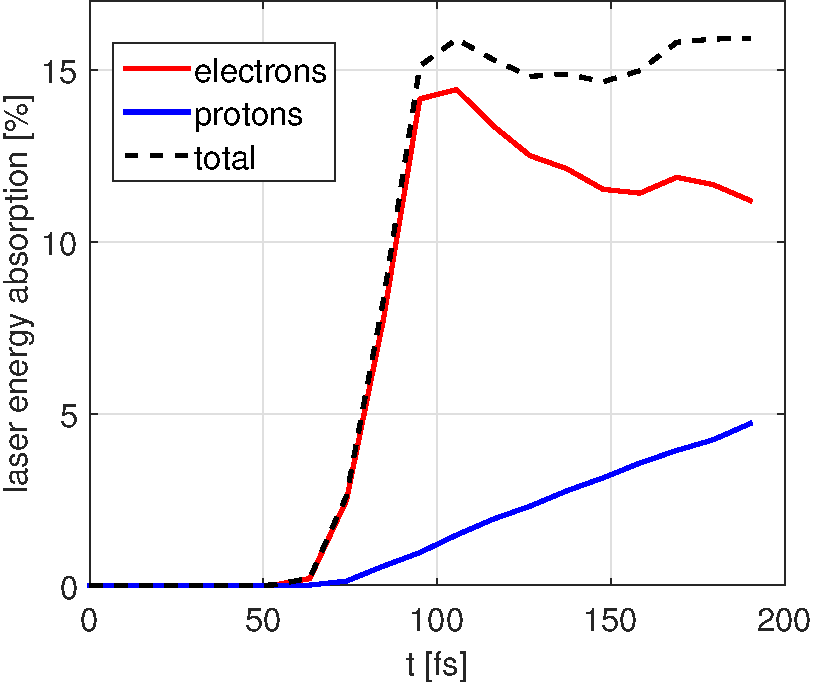
\includegraphics[width=0.45\linewidth]{./img/results/i1e20/05/absorp.pdf}}}
	\sidesubfloat[]{{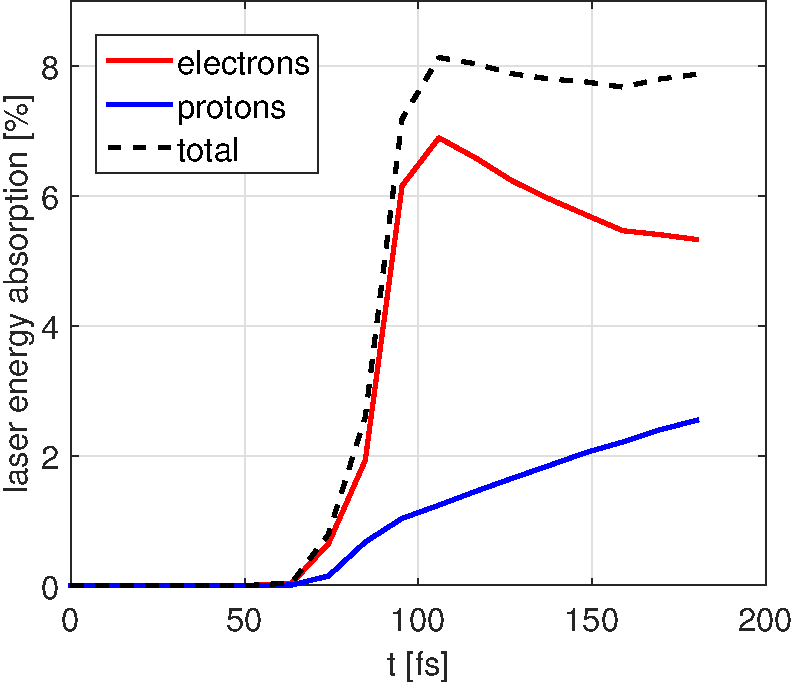
\includegraphics[width=0.45\linewidth]{./img/results/i1e20/2/absorp.pdf}}}\\
	\sidesubfloat[]{{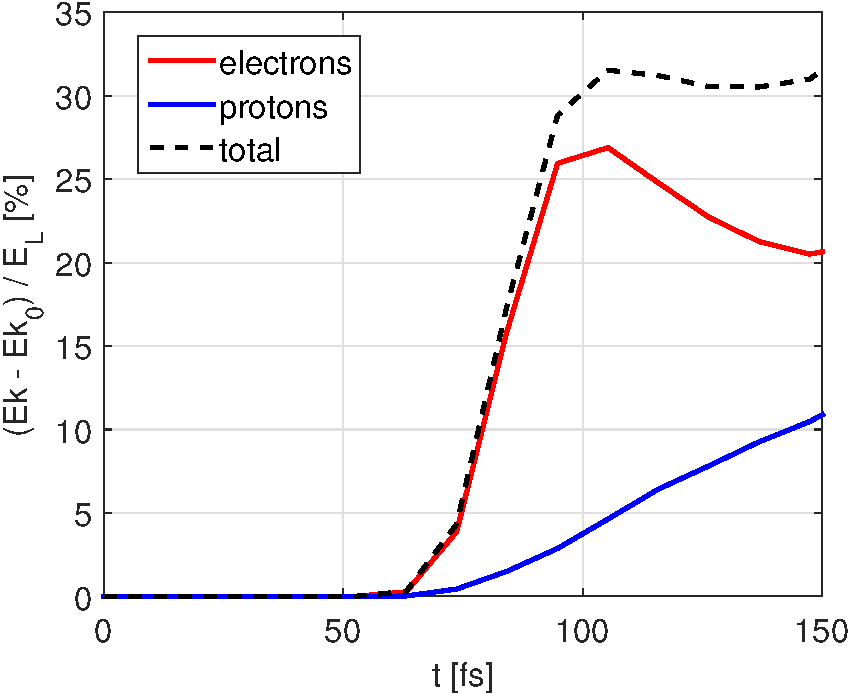
\includegraphics[width=0.45\linewidth]{./img/results/i1e21/05/absorp.pdf}}}
	\sidesubfloat[]{{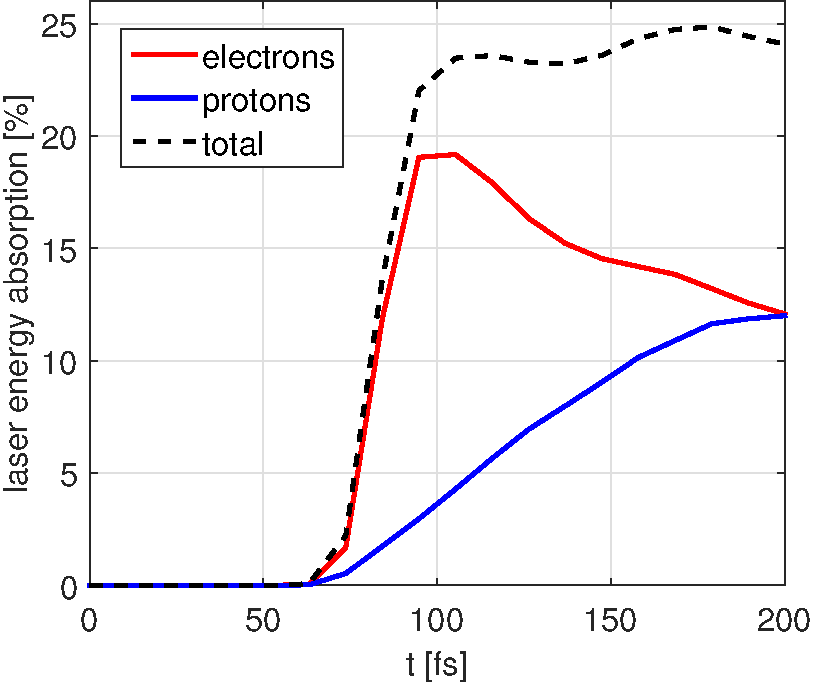
\includegraphics[width=0.45\linewidth]{./img/results/i1e21/2/absorp.pdf}}}
	\caption{The laser energy absorption in time for the case of simulations with the laser intensity $ I = 10^{20} \ \mathrm{W/cm^2} $ and with the beam waist \textbf{(a)} $ w_0 = 0.5 \ \mu\mathrm{m} $, \textbf{(b)} $ w_0 = 2.0 \ \mu\mathrm{m} $ and for the case of simulations with the laser intensity $ I = 10^{21} \ \mathrm{W/cm^2} $ and with the beam waist \textbf{(c)} $ w_0 = 0.5 \ \mu\mathrm{m} $, \textbf{(d)} $ w_0 = 2.0 \ \mu\mathrm{m} $.}
	\label{fig:10}
\end{figure}

First, the results have been analyzed in terms of laser energy absorption efficiency. The comparison of rates of the total laser light absorption in plasma for all the simulations is shown in table \ref{table:2}. It might be clearly seen that for the simulations where the beam is focused to a focal spot larger than the center laser wavelength whilst its peak intensity remains the same, there is no significant difference between the absorption rates. On the other hand, in the case of the sub-wavelength level focus, the rate of energy absorption sharply increases. The difference of the absorption percentage between the beams focused to $ w_0 = 1.0 \ \mu\mathrm{m} $ and $ w_0 = 0.5 \ \mu\mathrm{m} $ is $ 6.64 \ \% $ in the case of laser intensity $ I = 10^{20} \ \mathrm{W/cm^2} $ and $ 8.01 \ \% $ in the case of intensity $ I = 10^{21} \ \mathrm{W/cm^2} $.

\floatsetup[figure]{style=plain, subcapbesideposition=top}
\begin{figure}[h!]
	\centering
	\sidesubfloat[]{{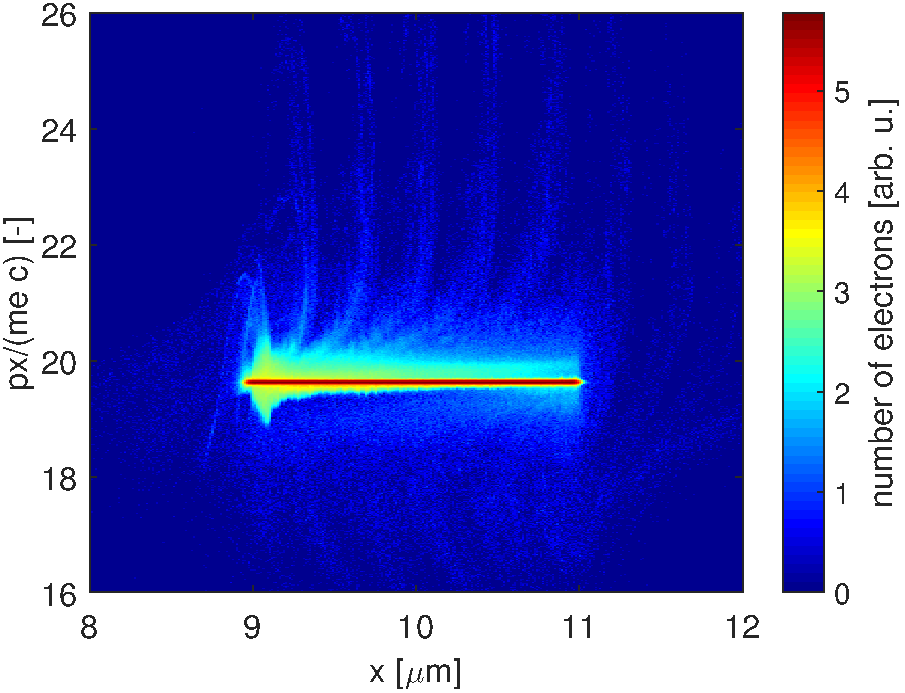
\includegraphics[width=0.45\linewidth]{./img/results/i1e20/05/x_px.pdf}}}
	\sidesubfloat[]{{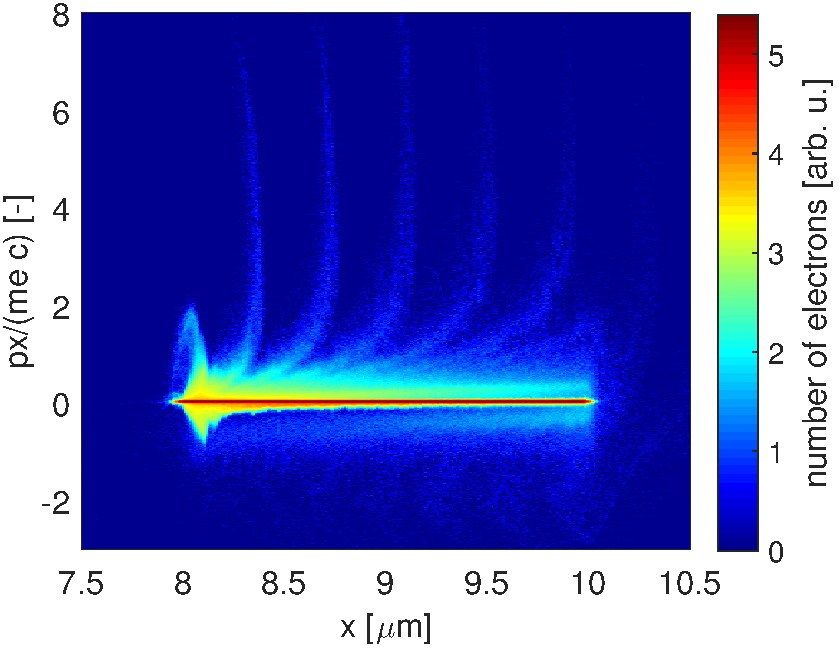
\includegraphics[width=0.45\linewidth]{./img/results/i1e20/2/x_px.pdf}}}\\
	\sidesubfloat[]{{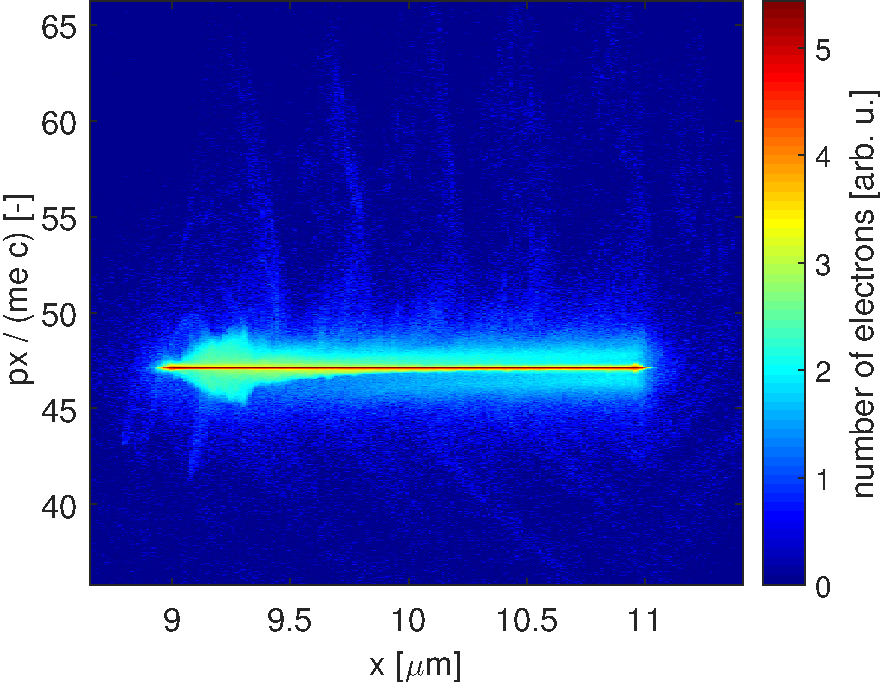
\includegraphics[width=0.45\linewidth]{./img/results/i1e21/05/x_px.pdf}}}
	\sidesubfloat[]{{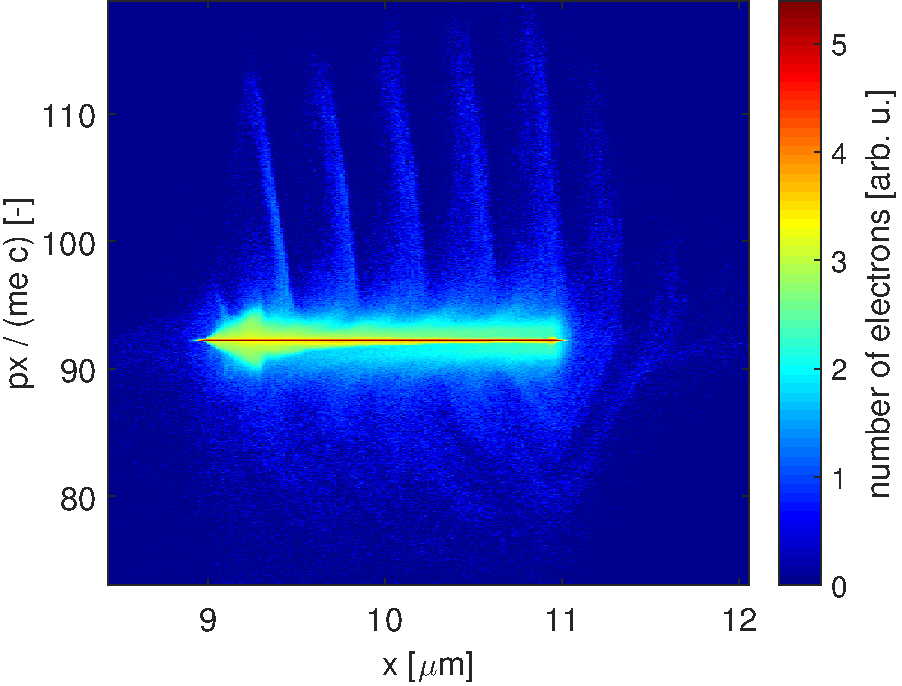
\includegraphics[width=0.45\linewidth]{./img/results/i1e21/2/x_px.pdf}}}
	\caption{The phase space of the parallel component of the momentum ($ p_x $) and the x-coordinate of all electrons in the simulation domain at the time $ t = 100 \ \mathrm{fs} $ for the case of simulations with the laser intensity $ I = 10^{20} \ \mathrm{W/cm^2} $ and with the beam waist \textbf{(a)} $ w_0 = 0.5 \ \mu\mathrm{m} $, \textbf{(b)} $ w_0 = 2.0 \ \mu\mathrm{m} $ and for the case of simulations with the laser intensity $ I = 10^{21} \ \mathrm{W/cm^2} $ and with the beam waist \textbf{(c)} $ w_0 = 0.5 \ \mu\mathrm{m} $, \textbf{(d)} $ w_0 = 2.0 \ \mu\mathrm{m} $. The color scales are logarithmic and the units are arbitrary, but the same for all sub-figures.}
	\label{fig:11}
\end{figure}

In fig. \ref{fig:10}, one can see the instantaneous laser energy absorption rate with respect to time. The plots indicate that as the focal spot size increases, the energy transfer to ions is faster. This can be explained by the fact that the amount of electrons recirculating in plasma is proportional to the size of the laser focus. Also, one may expect that the processes responsible for energy transfer that take place during the interaction will be similar. Therefore, one shall identify the main plasma heating and energy absorption mechanisms.

\floatsetup[figure]{style=plain, subcapbesideposition=top}
\begin{figure}[h!]
	\centering
	\sidesubfloat[]{{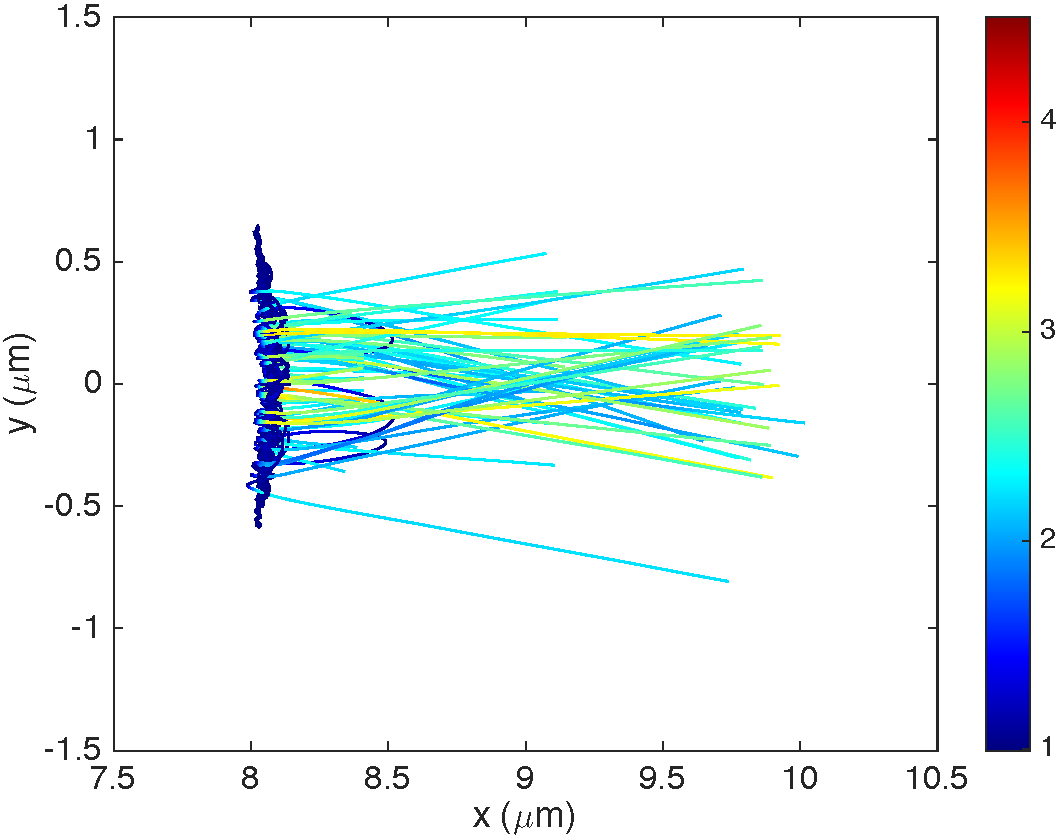
\includegraphics[width=0.4\linewidth]{./img/results/i1e20/05/traj_1.pdf}}}
	\sidesubfloat[]{{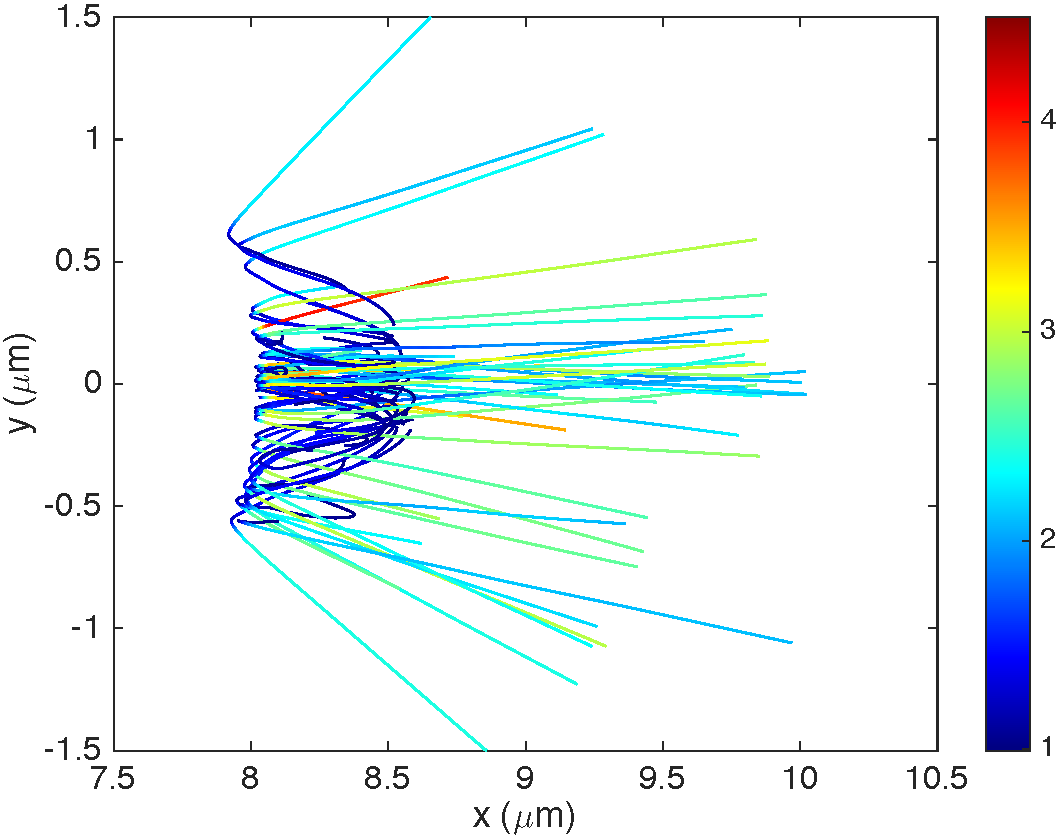
\includegraphics[width=0.4\linewidth]{./img/results/i1e20/05/traj_2.pdf}}}\\[2mm]
	\sidesubfloat[]{{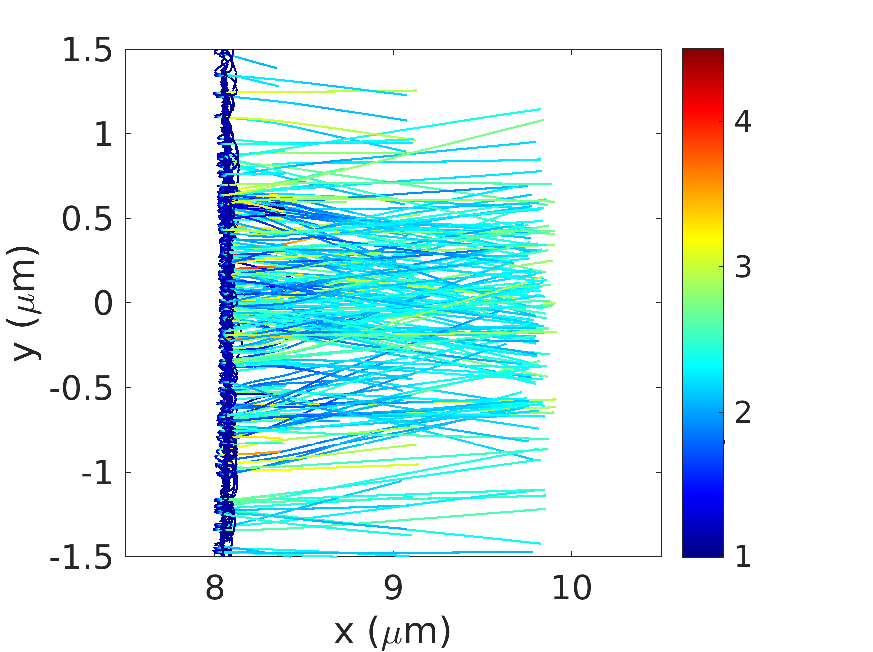
\includegraphics[width=0.4\linewidth]{./img/results/i1e20/2/traj_1.pdf}}}
	\sidesubfloat[]{{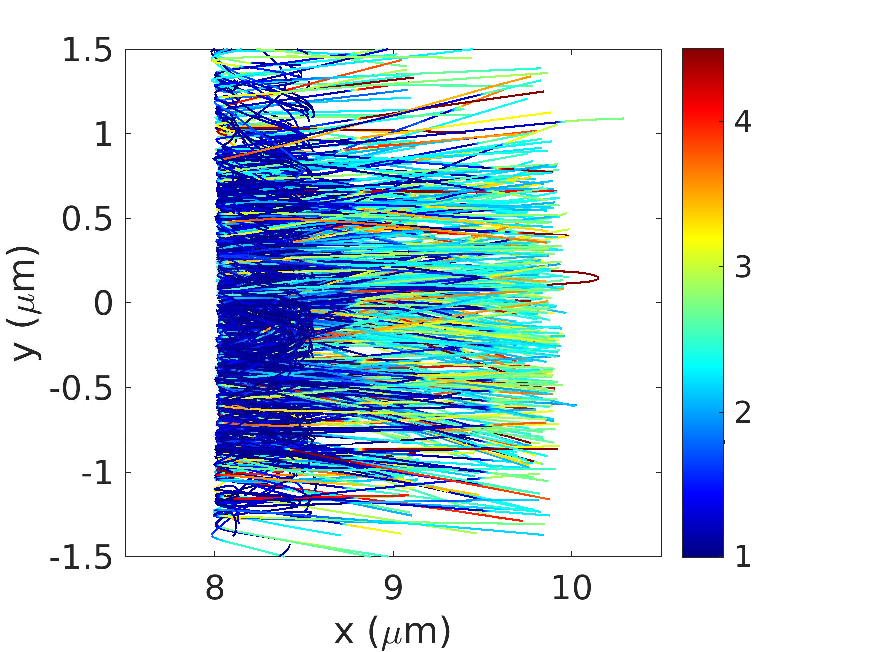
\includegraphics[width=0.4\linewidth]{./img/results/i1e20/2/traj_2.pdf}}}
	\caption{Two types of trajectories of randomly chosen electron samples for the case of simulations with the laser intensity $ I = 10^{20} \ \mathrm{W/cm^2} $ and with the beam waist \textbf{(a), (b)} $ w_0 = 0.5 \ \mu\mathrm{m} $ and \textbf{(c), (d)} $ w_0 = 2.0 \ \mu\mathrm{m} $. The trajectories are colored according to the Lorentz gamma factor of corresponding particles.}
	\label{fig:19}
\end{figure}

Regarding the laser intensities, one expects that the dominating absorption mechanism is $ \vec{J} \times \vec{B} $ heating. The phase space of the parallel component of the momentum and the x-coordinate of all electrons in the simulation domain at the time $ t = 100 \ \mathrm{fs} $ is shown in fig. \ref{fig:11}. The bunches of hot electrons that are ejected twice per laser period indicate that the $ \vec{J} \times \vec{B} $ heating is much more efficient in the case of $ w_0 = 2.0 \ \mu\mathrm{m} $ where the peak longitudinal momentum $ p_x \approx 8 \ m_{e} c $ in the case of laser intensity $ I = 10^{20} \ \mathrm{W/cm^2} $ (fig. \ref{fig:11}-b) and $ p_x \approx 22 \ m_{e} c $ in the case of intensity $ I = 10^{21} \ \mathrm{W/cm^2} $ (fig. \ref{fig:11}-d). Thus, to better understand the absorption mechanisms that take place during the interaction in the case of $ w_0 = 0.5 \ \mu\mathrm{m} $, it is necessary to perform further investigations.

For deeper understanding, it might be useful to track particle trajectories. For this reason, the fig. \ref{fig:19} shows trajectories of randomly chosen electron samples for the laser intensity $ I = 10^{20} \ \mathrm{W/cm^2} $. It turned out, that most of the trajectories can be split up into two groups. The first type of trajectories corresponds to electrons that move along the front surface of the target towards the focal spot and in the vicinity of the focus, these electrons are pushed into the target in a highly collimated beam (fig. \ref{fig:19}-a, \ref{fig:19}-c). The second type of trajectories corresponds to electrons that are initially inside the target, then they are ejected at the target front surface and pushed back to the plasma in a relatively divergent beam (fig. \ref{fig:19}-b, \ref{fig:19}-d). 

\floatsetup[figure]{style=plain, subcapbesideposition=top}
\begin{figure}[h!]
	\centering
	\sidesubfloat[]{{\includegraphics[width=0.45\linewidth]{./img/results/i1e20/05/fpx.pdf}}}
	\sidesubfloat[]{{\includegraphics[width=0.45\linewidth]{./img/results/i1e20/05/fpy.pdf}}}\\
	\sidesubfloat[]{{\includegraphics[width=0.45\linewidth]{./img/results/i1e20/2/fpx.pdf}}}
	\sidesubfloat[]{{\includegraphics[width=0.45\linewidth]{./img/results/i1e20/2/fpy.pdf}}}
	\caption{The longitudinal ($ F_{\mathrm{p}, x} $) \textbf{(a)} and the transverse ($ F_{\mathrm{p}, y} $) \textbf{(b)} component of the ponderomotive force for the case of the laser beam with intensity $ I = 10^{20} \ \mathrm{W/cm^2} $ and the beam waist $ w_0 = 0.5 \ \mu\mathrm{m} $ propagating in vacuum. The longitudinal ($ F_{\mathrm{p}, x} $) \textbf{(c)} and the transverse ($ F_{\mathrm{p}, y} $) \textbf{(d)} component of the ponderomotive force for the case of the laser beam with intensity $ I = 10^{20} \ \mathrm{W/cm^2} $ and the beam waist $ w_0 = 2.0 \ \mu\mathrm{m} $ propagating in vacuum. The ponderomotive force has been calculated according to the non-relativistic formula \ref{2.5.1.11}.}
	\label{fig:21}
\end{figure}

Note that there is significant quantitative difference between the two focal spot sizes for both trajectories. In the case of $ w_0 = 0.5 \ \mu\mathrm{m} $, there is approximately $ 59 \ \% $ of electrons with the trajectories of the first type (fig. \ref{fig:19}-a) and $ 41 \ \% $ of the second type (fig. \ref{fig:19}-b). On the contrary, for the simulation of $ w_0 = 2.0 \ \mu\mathrm{m} $, there is about $ 22 \ \% $ of electrons with the trajectories of the first type (fig. \ref{fig:19}-c) and $ 78 \ \% $ of the second type (fig. \ref{fig:19}-d).

\floatsetup[figure]{style=plain, subcapbesideposition=top}
\begin{figure}[h!]
	\centering
	\sidesubfloat[]{{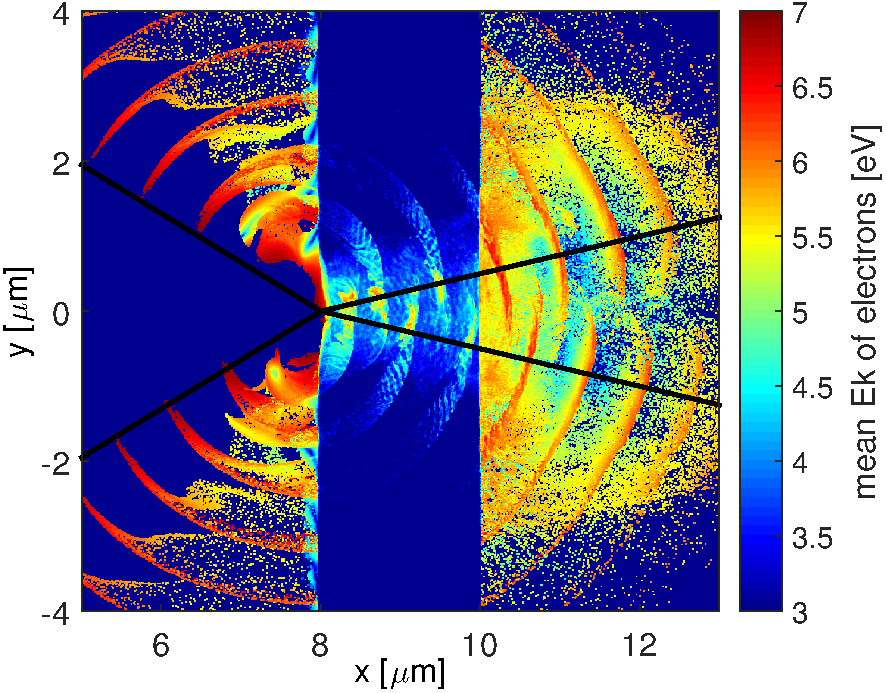
\includegraphics[width=0.45\linewidth]{./img/results/i1e21/05/ekbar_2.pdf}}}
	\sidesubfloat[]{{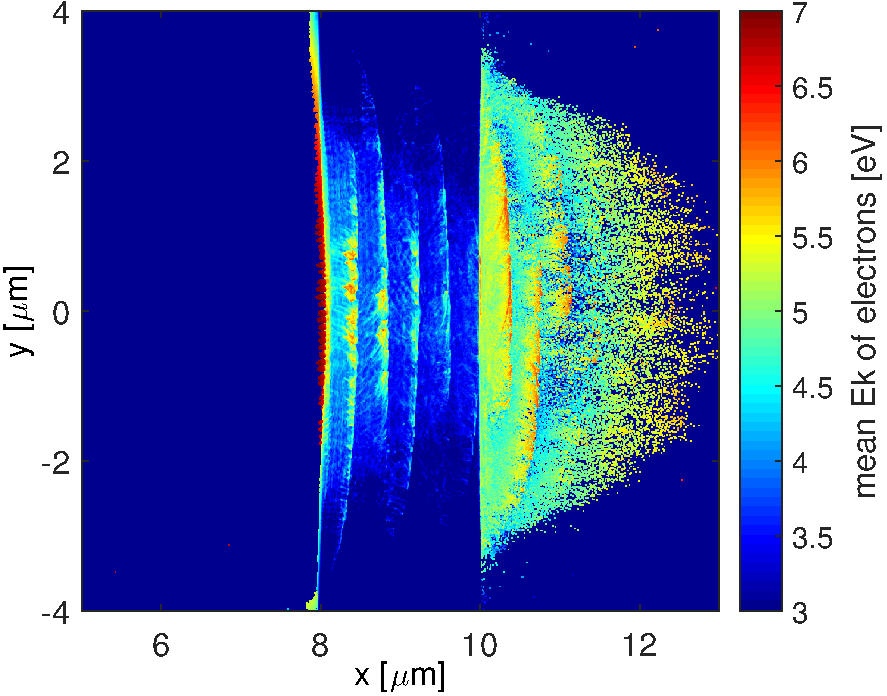
\includegraphics[width=0.45\linewidth]{./img/results/i1e21/2/ekbar_2.pdf}}}\\[2mm]
	\caption{Mean kinetic energy of electrons at the time $ t = 80 \ \mathrm{fs} $ for the case of simulations with the laser intensity $ I = 10^{21} \ \mathrm{W/cm^2} $ and with the beam waist \textbf{(a)} $ w_0 = 0.5 \ \mu\mathrm{m} $, \textbf{(b)} $ w_0 = 2.0 \ \mu\mathrm{m} $. The color scales are logarithmic.}
	\label{fig:17}
\end{figure}

\floatsetup[figure]{style=plain, subcapbesideposition=top}
\begin{figure}[h!]
	\centering
	\sidesubfloat[]{{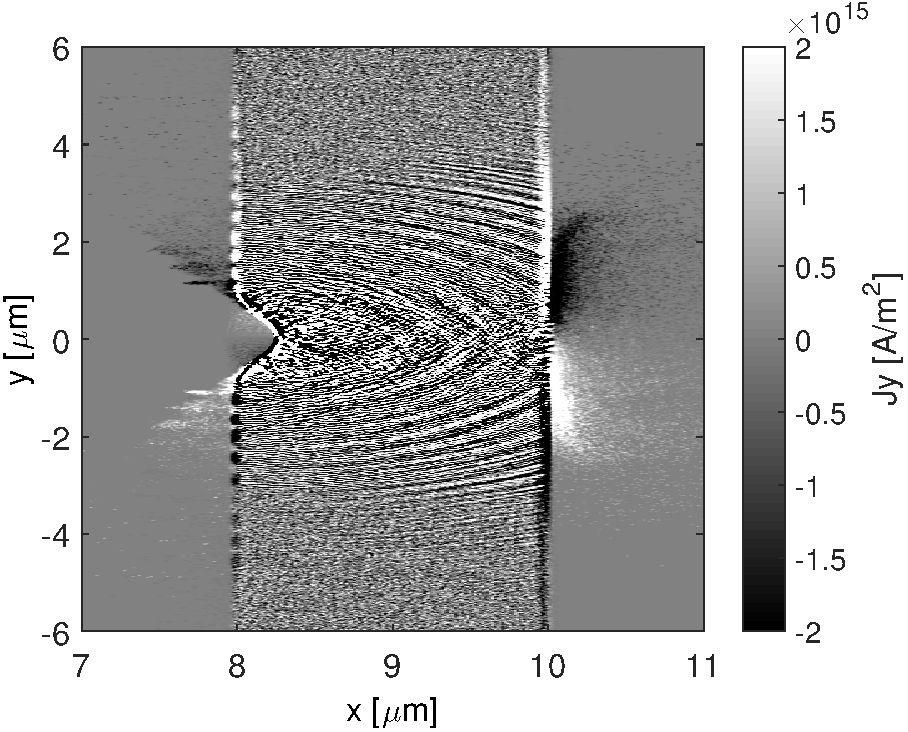
\includegraphics[width=0.45\linewidth]{./img/results/i1e21/05/jy.pdf}}}
	\sidesubfloat[]{{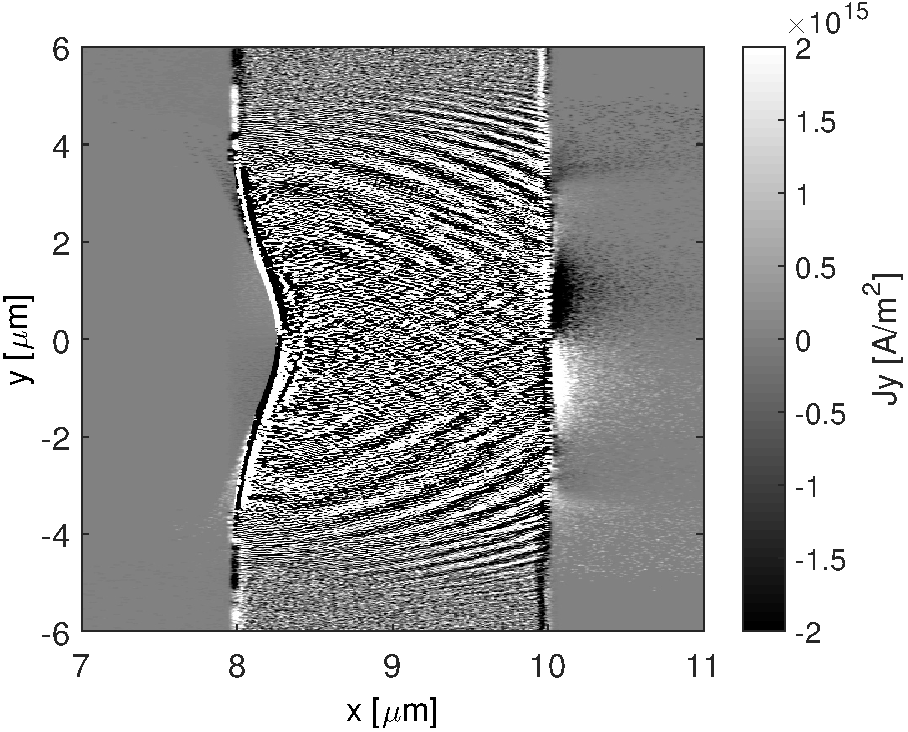
\includegraphics[width=0.45\linewidth]{./img/results/i1e21/2/jy.pdf}}}\\[2mm]
	\caption{Perpendicular component of the current density $ J_{y} $ at the time $ t = 100 \ \mathrm{fs} $ for the case of simulations with the laser intensity $ I = 10^{21} \ \mathrm{W/cm^2} $ and with the beam waist \textbf{(a)} $ w_0 = 0.5 \ \mu\mathrm{m} $, \textbf{(b)} $ w_0 = 2.0 \ \mu\mathrm{m} $.}
	\label{fig:18}
\end{figure}

The electron trajectories are determined mainly by the laser field. In fig. \ref{fig:21}, one can see the longitudinal and transverse components of the ponderomotive force for the laser beam with intensity $ I = 10^{20} \ \mathrm{W/cm^2} $ and focal spot sizes $ w_0 = 0.5, 2.0 \ \mu\mathrm{m} $ propagating in vacuum. The magnitude of longitudinal component is comparable for both cases, but the transverse component is approximately $ 3.5 $ times higher in the case of $ w_0 = 0.5 \ \mu\mathrm{m} $. The ratio of longitudinal component of the ponderomotive force to transverse is approximately $ 3.2:1 $ in the case of $ w_0 = 0.5 \ \mu\mathrm{m} $ and $ 12.8:1 $ in the case of $ w_0 = 2.0 \ \mu\mathrm{m} $. Note that for the laser intensity $ I = 10^{21} \ \mathrm{W/cm^2} $, the ponderomotive force is $ 10 $ times higher, but the ratios remain the same.

\floatsetup[figure]{style=plain, subcapbesideposition=top}
\begin{figure}[h!]
	\centering
	\sidesubfloat[]{{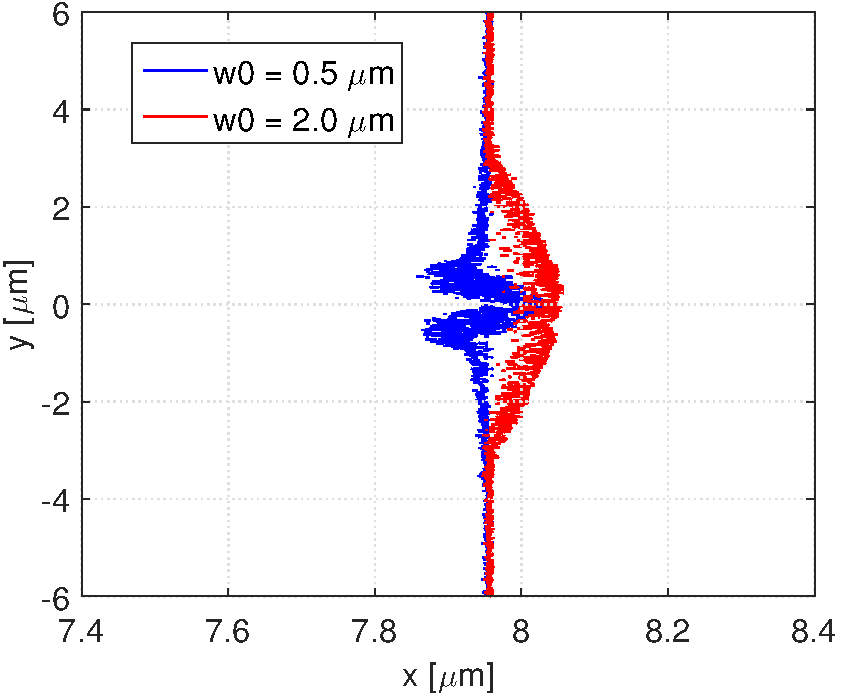
\includegraphics[width=0.445\linewidth]{./img/results/i1e20/dens.pdf}}}
	\hspace{1mm}
	\sidesubfloat[]{{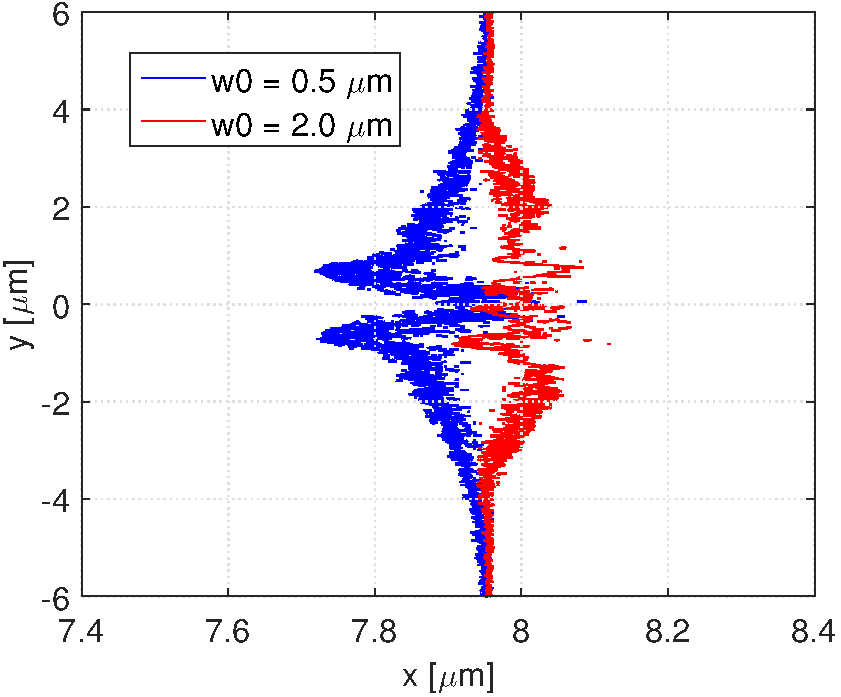
\includegraphics[width=0.445\linewidth]{./img/results/i1e21/dens.pdf}}}
	\caption{A contour lines of ion critical density for two different beam waists at the time $ t = 100 \ \mathrm{fs} $ for the case of simulations with the laser intensity \textbf{(a)} $ I = 10^{20} \ \mathrm{W/cm^2} $ and \textbf{(b)} $ I = 10^{21} \ \mathrm{W/cm^2} $.}
	\label{fig:15}
\end{figure}

The mean kinetic energy of electrons at the time $ t = 80 \ \mathrm{fs} $ is shown in fig. \ref{fig:17}. The divergence angle of electrons moving forward is given by the ratio of longitudinal component of the ponderomotive force to the transverse component. In the case of $ w_0 = 0.5 \ \mu\mathrm{m} $, the divergence angle (marked by a black line in fig. \ref{fig:17}-a) is estimated to $ 33^{\circ} $, whilst in the case of $ w_0 = 2.0 \ \mu\mathrm{m} $, the divergence angle is only $ 9^{\circ} $. In both cases, one may see the bunches of hot electrons that are ejected twice per laser period. In addition, in the case of $ w_0 = 0.5 \ \mu\mathrm{m} $, one may also clearly see the electrons that move backwards. Their movement is restricted by the incoming laser beam (the laser divergence angle is marked off by a black line in front of the target in fig. \ref{fig:17}-a).

The perpendicular component of the current density at the time $ t = 100 \ \mathrm{fs} $ is shown in fig. \ref{fig:18}. In the case of $ w_0 = 0.5 \ \mu\mathrm{m} $ (fig. \ref{fig:18}-a), one may register the electric current caused by the electrons ejected into vacuum. The charge unbalance is then compensated by the electric current along the front surface and this might be the reason, why there is more electrons with the trajectories of the first type.

The fig. \ref{fig:18} also indicates different shape of the target deformed during the hole boring phase. For this reason, a contour lines of ion critical density are shown in the fig. \ref{fig:15}. Notice that in the case of $ w_0 = 0.5 \ \mu\mathrm{m} $, the plasma in the vicinity of incoming laser beam expands rapidly (marked by blue lines in fig. \ref{fig:15}-a, \ref{fig:15}-b). It means that the absorption processes which take place when the laser pulse is obliquely incident on a plasma density gradient (such as resonance absorption) may also significantly contribute to overall absorption.

The mean kinetic energy of electrons at the time $ t = 120 \ \mathrm{fs} $ in a global view is shown in fig. \ref{fig:16}. One can clearly see that in the case of $ w_0 = 0.5 \ \mu\mathrm{m} $, 

\floatsetup[figure]{style=plain, subcapbesideposition=top}
\begin{figure}[h!]
	\centering
	\sidesubfloat[]{{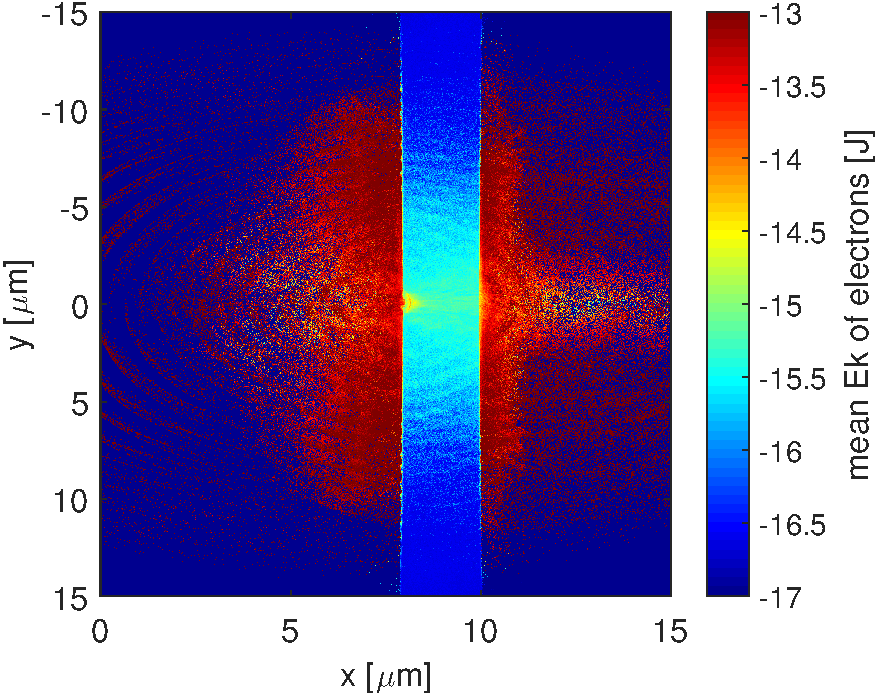
\includegraphics[width=0.45\linewidth]{./img/results/i1e20/05/ekbar.pdf}}}
	\sidesubfloat[]{{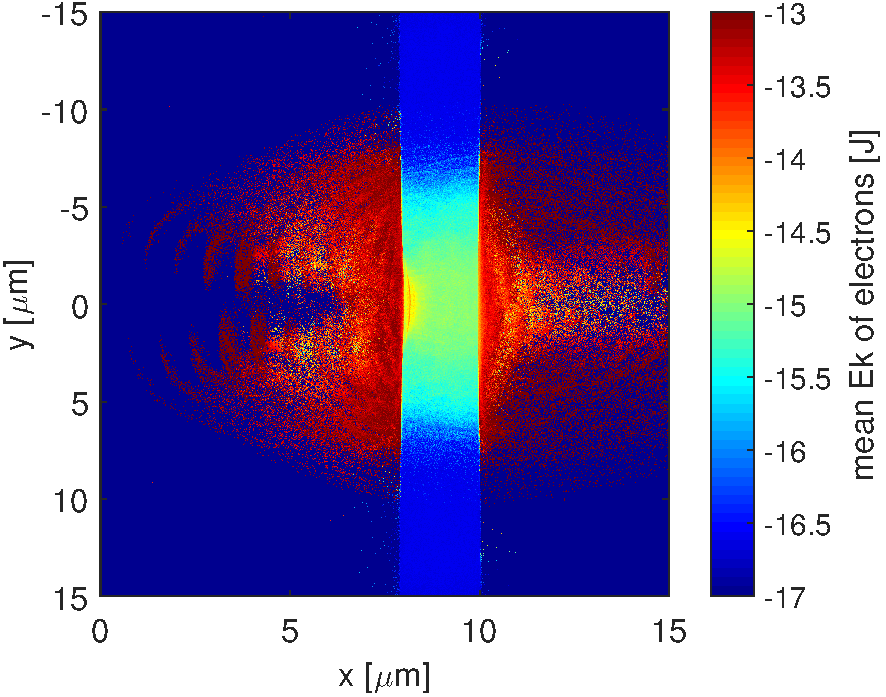
\includegraphics[width=0.45\linewidth]{./img/results/i1e20/2/ekbar.pdf}}}\\[2mm]
	\sidesubfloat[]{{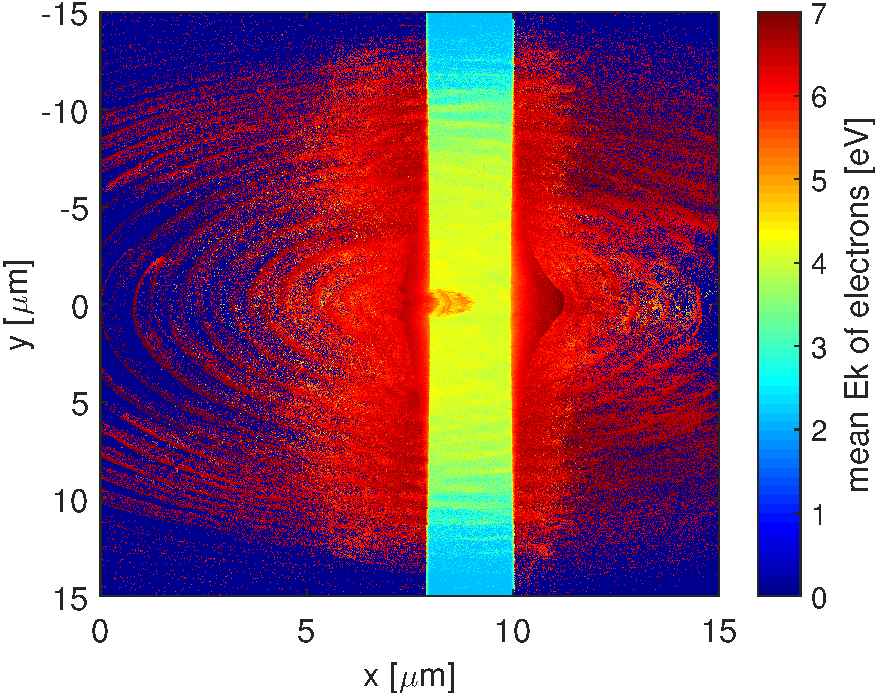
\includegraphics[width=0.45\linewidth]{./img/results/i1e21/05/ekbar.pdf}}}
	\sidesubfloat[]{{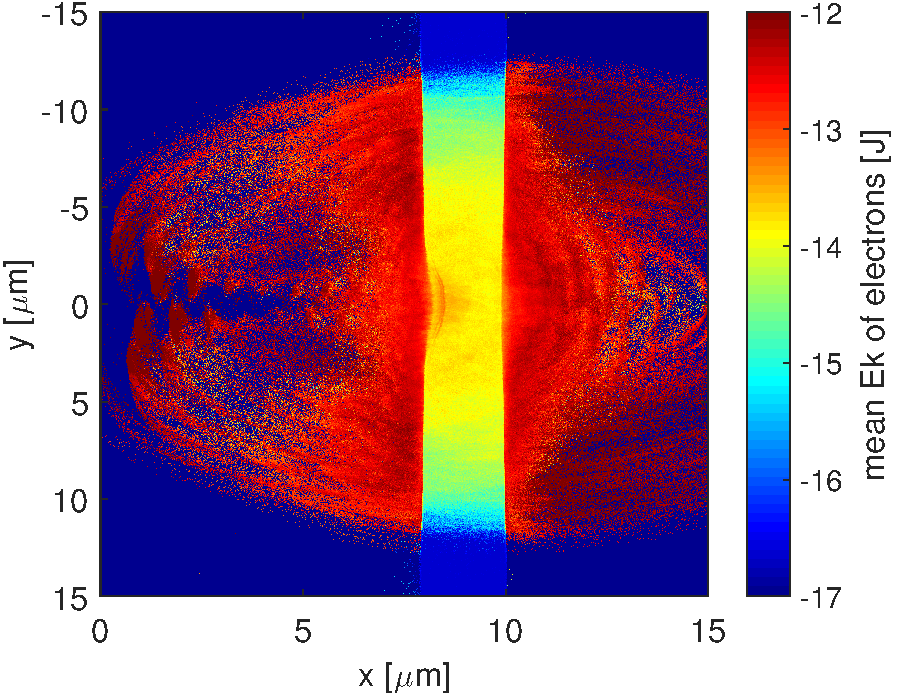
\includegraphics[width=0.45\linewidth]{./img/results/i1e21/2/ekbar.pdf}}}
	\caption{Mean kinetic energy of electrons at the time $ t = 120 \ \mathrm{fs} $ for the case of simulations with the laser intensity $ I = 10^{20} \ \mathrm{W/cm^2} $ and with the beam waist \textbf{(a)} $ w_0 = 0.5 \ \mu\mathrm{m} $, \textbf{(b)} $ w_0 = 2.0 \ \mu\mathrm{m} $ and for the case of simulations with the laser intensity $ I = 10^{21} \ \mathrm{W/cm^2} $ and with the beam waist \textbf{(c)} $ w_0 = 0.5 \ \mu\mathrm{m} $, \textbf{(d)} $ w_0 = 2.0 \ \mu\mathrm{m} $. The color scales are logarithmic.}
	\label{fig:16}
\end{figure}

\floatsetup[figure]{style=plain, subcapbesideposition=top}
\begin{figure}[h!]
	\centering
	\sidesubfloat[]{{\includegraphics[width=0.45\linewidth]{./img/results/i1e20/05/abs_ex.pdf}}}
	\sidesubfloat[]{{\includegraphics[width=0.45\linewidth]{./img/results/i1e20/2/abs_ex.pdf}}}\\[2mm]
	\sidesubfloat[]{{\includegraphics[width=0.45\linewidth]{./img/results/i1e21/05/abs_ex.pdf}}}
	\sidesubfloat[]{{\includegraphics[width=0.45\linewidth]{./img/results/i1e21/2/abs_ex.pdf}}}
	\caption{Longitudinal component of the electric field ($ E_{x} $) at the time  $ t = 120 \ \mathrm{fs} $ for the case of simulations with the laser intensity $ I = 10^{20} \ \mathrm{W/cm^2} $ and with the beam waist \textbf{(a)} $ w_0 = 0.5 \ \mu\mathrm{m} $, \textbf{(b)} $ w_0 = 2.0 \ \mu\mathrm{m} $ and for the case of simulations with the laser intensity $ I = 10^{21} \ \mathrm{W/cm^2} $ and with the beam waist \textbf{(c)} $ w_0 = 0.5 \ \mu\mathrm{m} $, \textbf{(d)} $ w_0 = 2.0 \ \mu\mathrm{m} $. Note that for $ w_0 = 2.0 \ \mu\mathrm{m} $ the color scales are saturated, thus the peak values are higher.}
	\label{fig:20}
\end{figure}

\floatsetup[figure]{style=plain, subcapbesideposition=top}
\begin{figure}[h!]
	\centering
	\sidesubfloat[]{{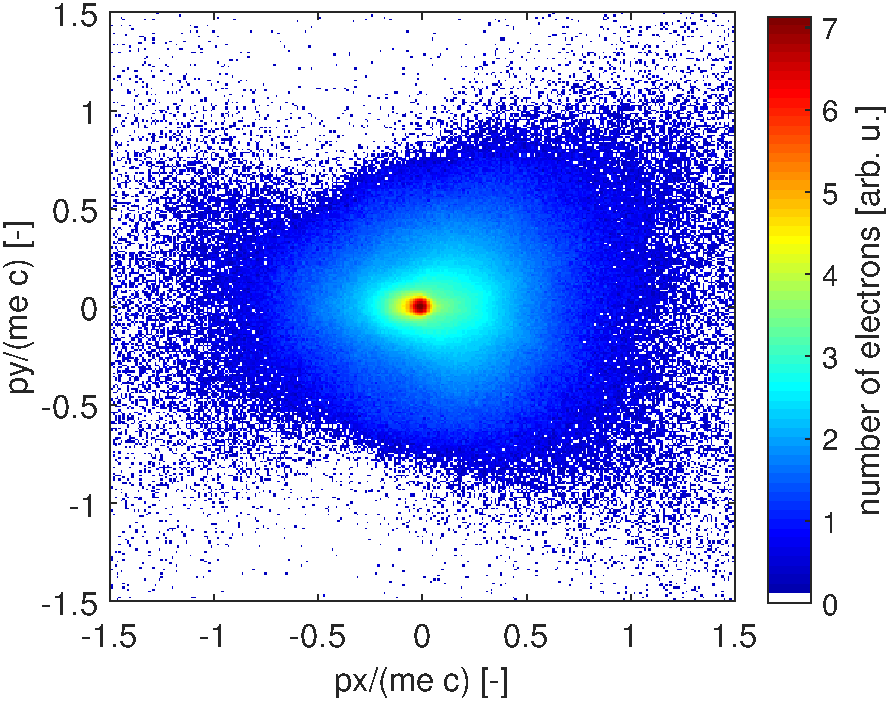
\includegraphics[width=0.45\linewidth]{./img/results/i1e20/05/px_py.pdf}}}
	\sidesubfloat[]{{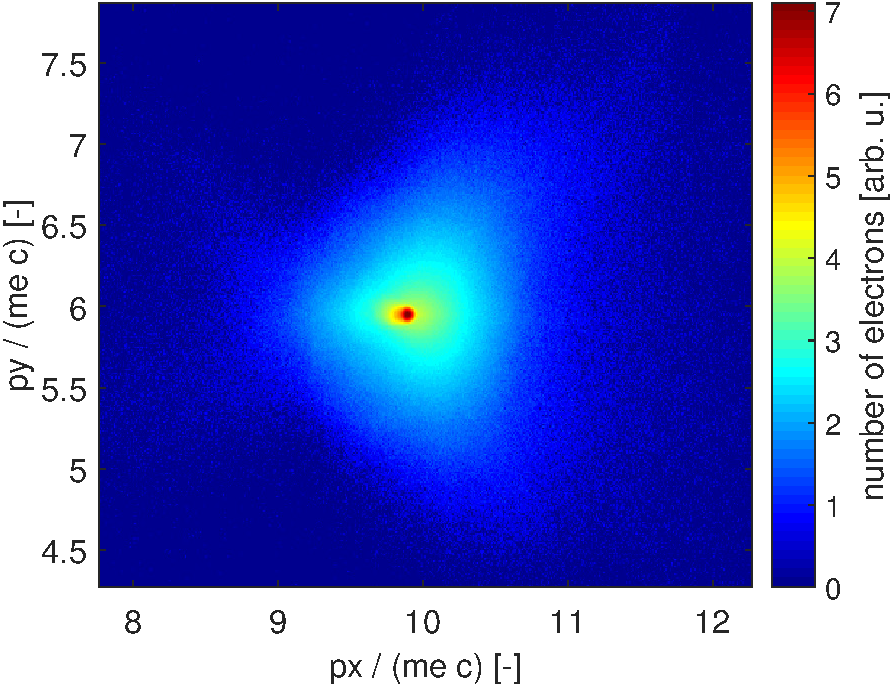
\includegraphics[width=0.45\linewidth]{./img/results/i1e20/2/px_py.pdf}}}\\
	\sidesubfloat[]{{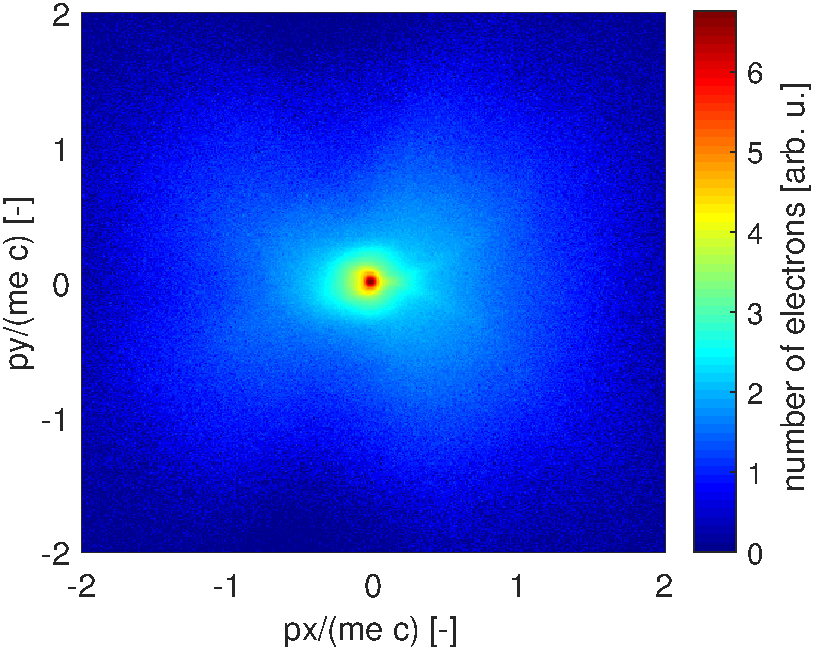
\includegraphics[width=0.45\linewidth]{./img/results/i1e21/05/px_py.pdf}}}
	\sidesubfloat[]{{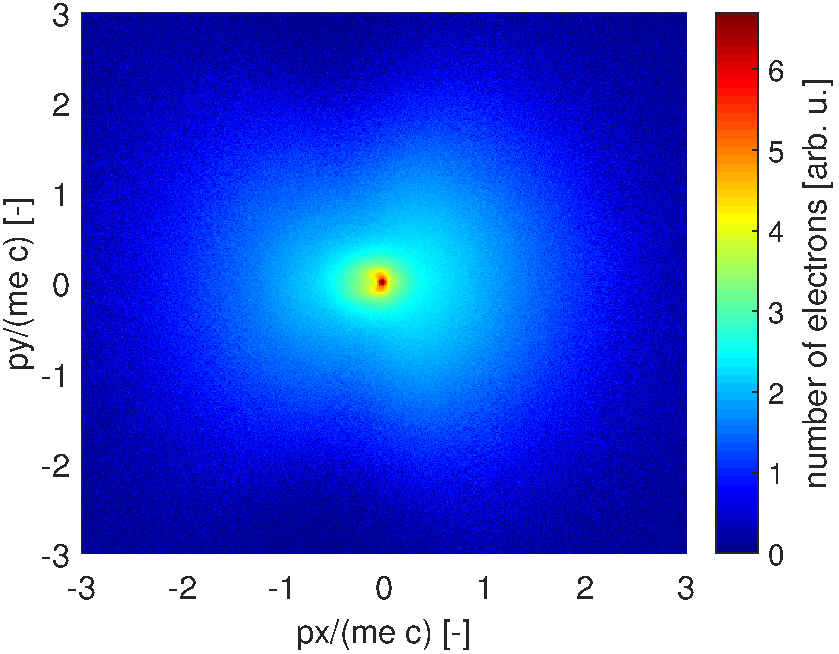
\includegraphics[width=0.45\linewidth]{./img/results/i1e21/2/px_py.pdf}}}
	\caption{Phase space of the parallel ($ p_x $) and the perpendicular ($ p_y $) components of the momentum of all electrons in the simulation domain at the time $ t = 100 \ \mathrm{fs} $ for the case of simulations with the laser intensity $ I = 10^{20} \ \mathrm{W/cm^2} $ and with the beam waist \textbf{(a)} $ w_0 = 0.5 \ \mu\mathrm{m} $, \textbf{(b)} $ w_0 = 2.0 \ \mu\mathrm{m} $ and for the case of simulations with the laser intensity $ I = 10^{21} \ \mathrm{W/cm^2} $ and with the beam waist \textbf{(c)} $ w_0 = 0.5 \ \mu\mathrm{m} $, \textbf{(d)} $ w_0 = 2.0 \ \mu\mathrm{m} $. The color scales are logarithmic and the units are arbitrary, but the same for all sub-figures.}
	\label{fig:12}
\end{figure}

\floatsetup[figure]{style=plain, subcapbesideposition=top}
\begin{figure}[h!]
	\centering
	\sidesubfloat[]{{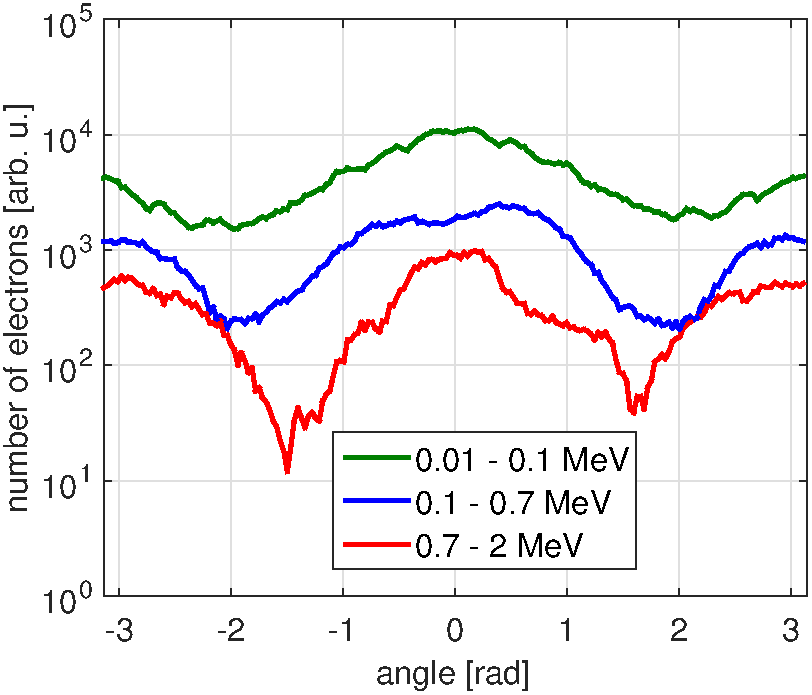
\includegraphics[width=0.445\linewidth]{./img/results/i1e20/05/angles.pdf}}}
	\hspace{1mm}
	\sidesubfloat[]{{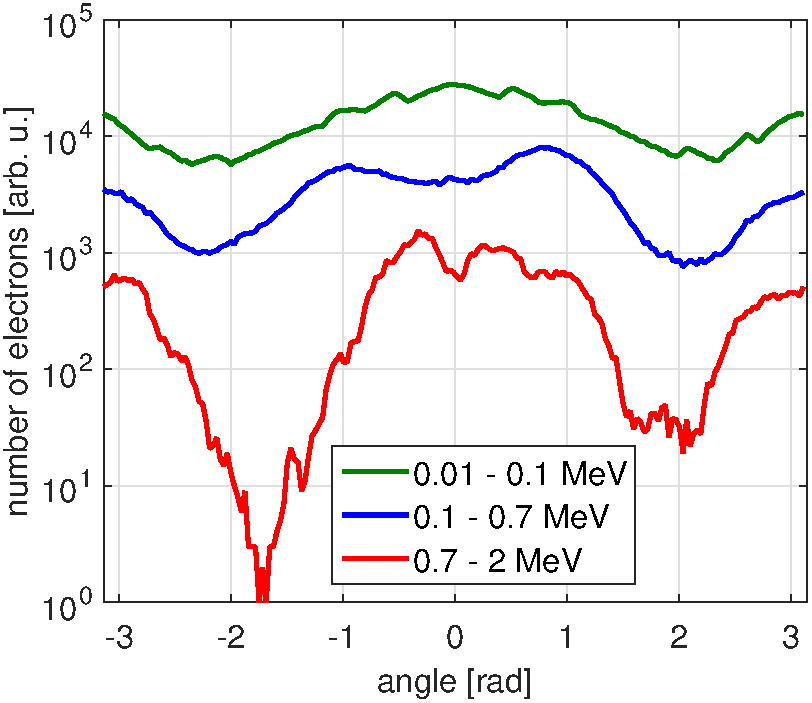
\includegraphics[width=0.445\linewidth]{./img/results/i1e20/2/angles.pdf}}}\\
	\sidesubfloat[]{{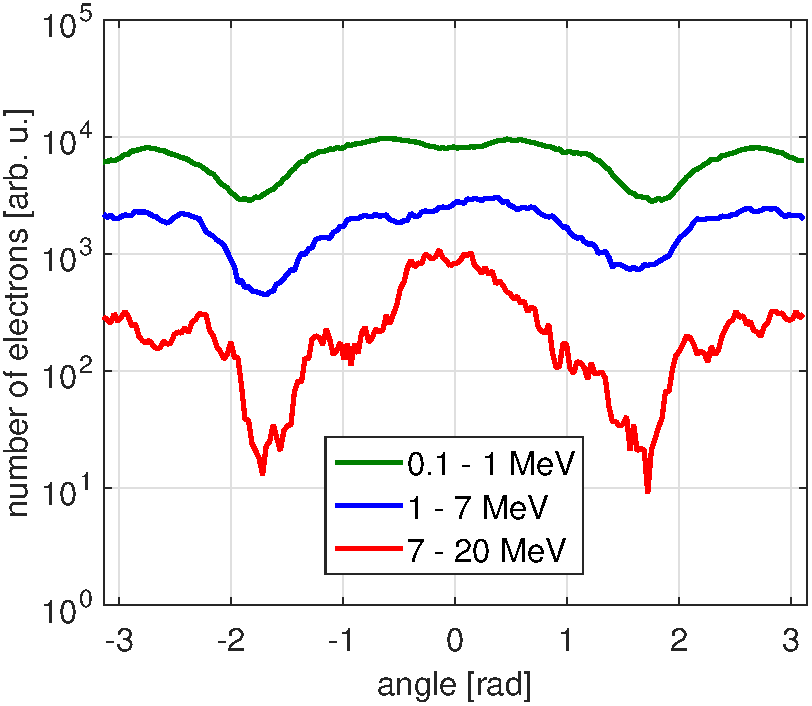
\includegraphics[width=0.445\linewidth]{./img/results/i1e21/05/angles.pdf}}}
	\hspace{1mm}
	\sidesubfloat[]{{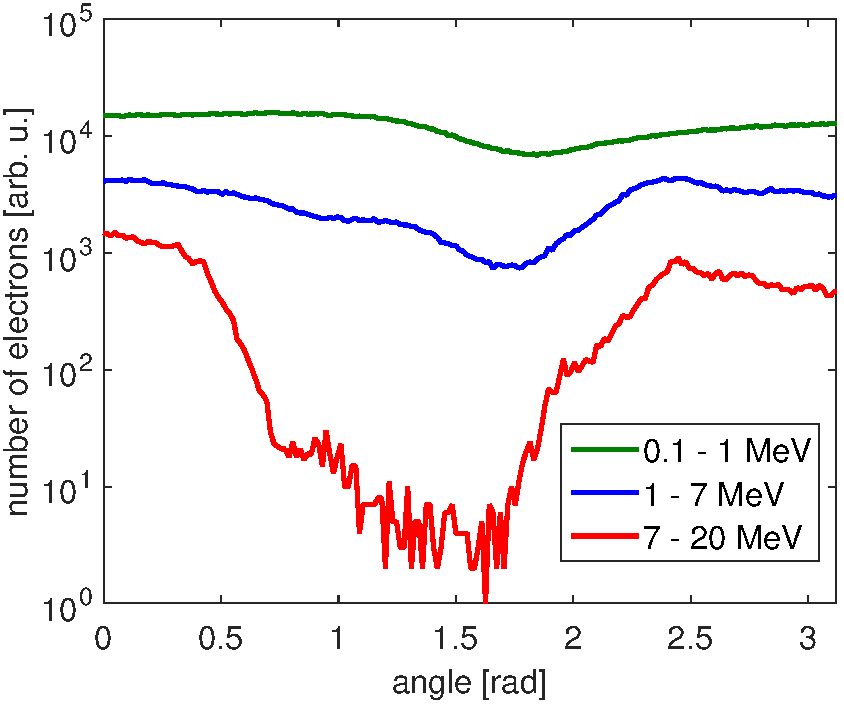
\includegraphics[width=0.445\linewidth]{./img/results/i1e21/2/angles.pdf}}}
	\caption{Angular distribution of electrons (the angle is measured with respect to the laser incidence direction) in the whole simulation domain at the time $ t = 100 \ \mathrm{fs} $ for the case of simulations with the laser intensity $ I = 10^{20} \ \mathrm{W/cm^2} $ and with the beam waist \textbf{(a)} $ w_0 = 0.5 \ \mu\mathrm{m} $, \textbf{(b)} $ w_0 = 2.0 \ \mu\mathrm{m} $ and for the case of simulations with the laser intensity $ I = 10^{21} \ \mathrm{W/cm^2} $ and with the beam waist \textbf{(c)} $ w_0 = 0.5 \ \mu\mathrm{m} $, \textbf{(d)} $ w_0 = 2.0 \ \mu\mathrm{m} $. The electrons are divided according to their kinetic energy into three separated intervals.}
	\label{fig:13}
\end{figure}

\floatsetup[figure]{style=plain, subcapbesideposition=top}
\begin{figure}[h!]
	\centering
	\sidesubfloat[]{{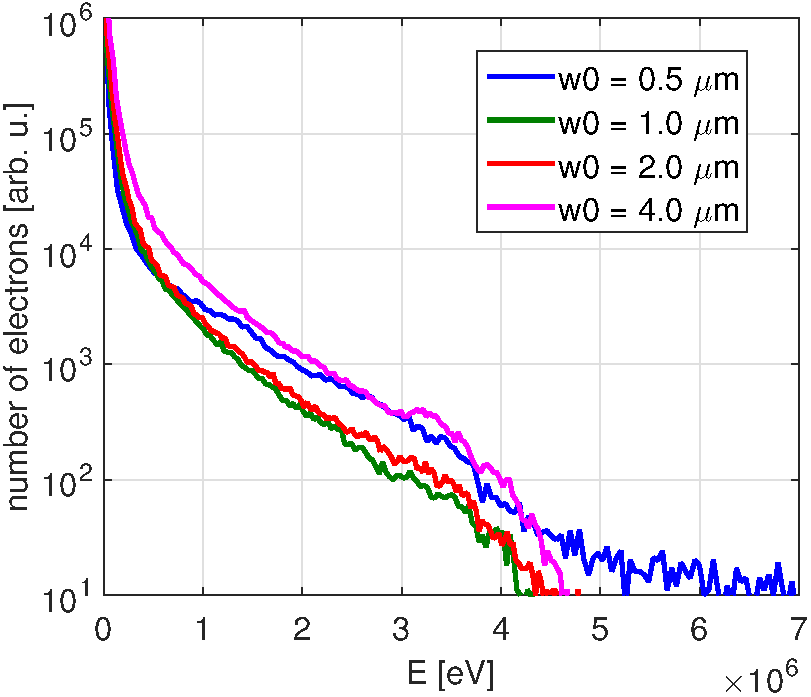
\includegraphics[width=0.445\linewidth]{./img/results/i1e20/dist_e.pdf}}}
	\hspace{1mm}
	\sidesubfloat[]{{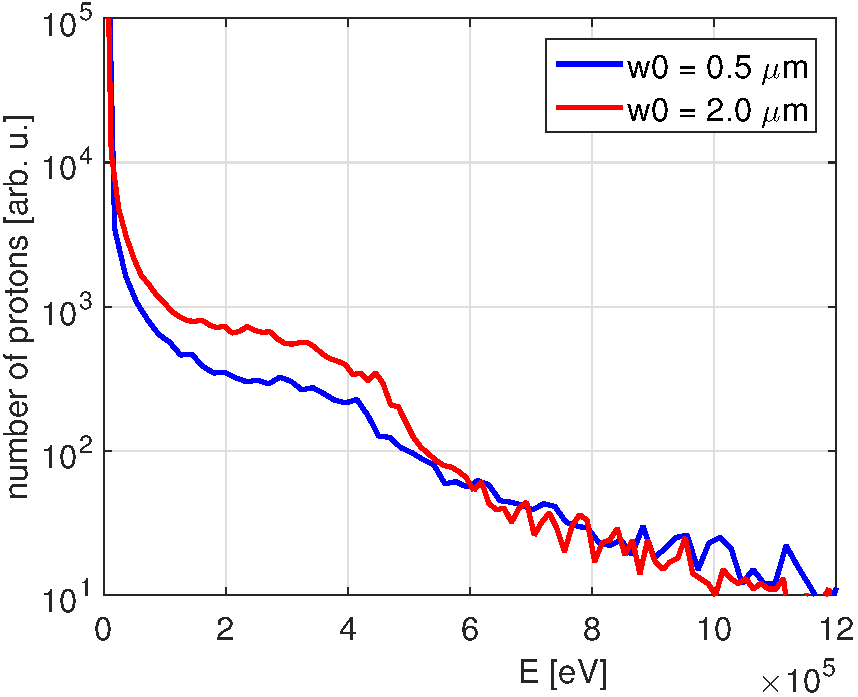
\includegraphics[width=0.445\linewidth]{./img/results/i1e20/dist_p.pdf}}}\\[2mm]
	\sidesubfloat[]{{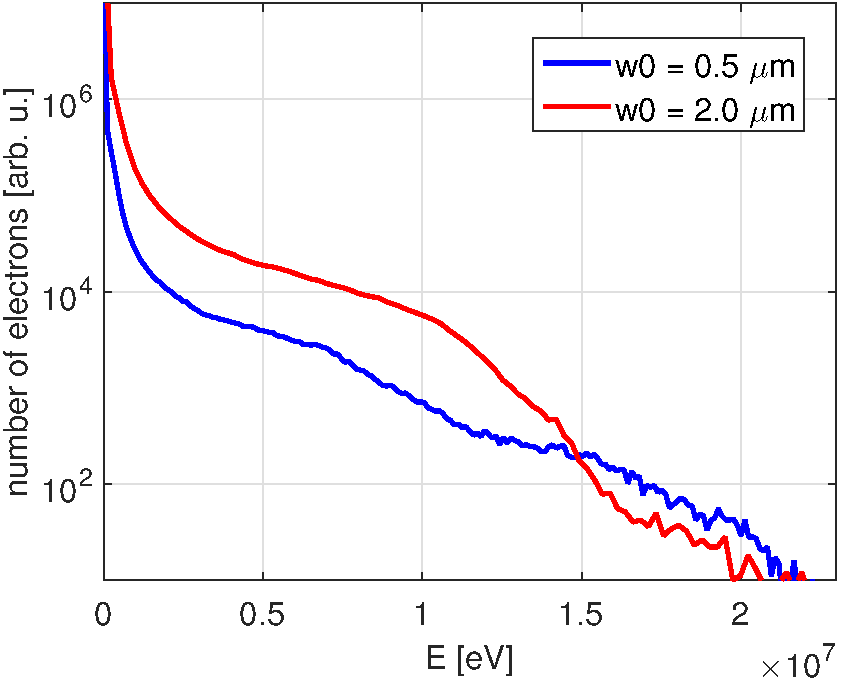
\includegraphics[width=0.445\linewidth]{./img/results/i1e21/dist_e.pdf}}}
	\hspace{1mm}
	\sidesubfloat[]{{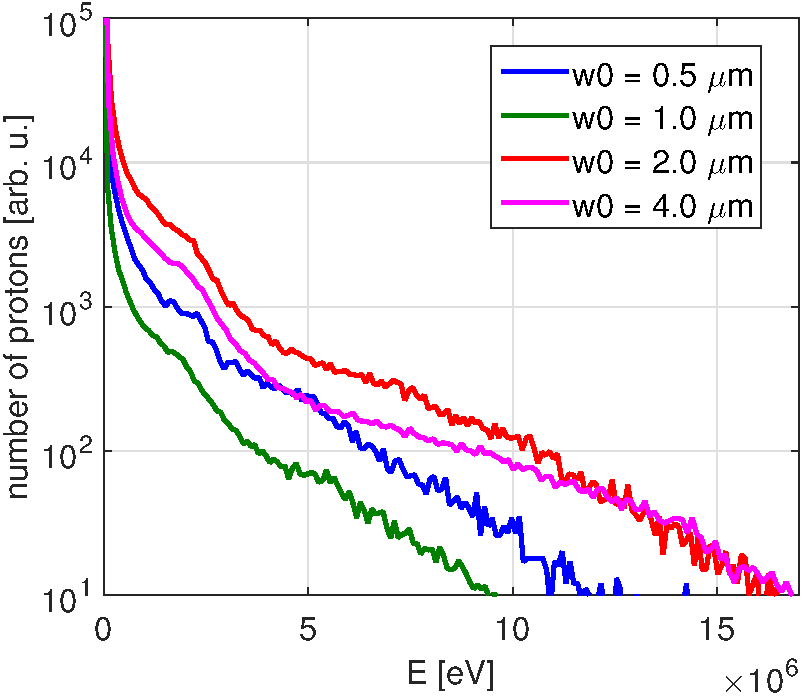
\includegraphics[width=0.445\linewidth]{./img/results/i1e21/dist_p.pdf}}}
	\caption{Electron energy distribution in the whole simulation domain for four different beam waists at the time $ t = 100 \ \mathrm{fs} $ for the case of simulations with the laser intensity \textbf{(a)} $ I = 10^{20} \ \mathrm{W/cm^2} $ and \textbf{(c)} $ I = 10^{21} \ \mathrm{W/cm^2} $. Ion energy distribution in the whole simulation domain for four different beam waists at the time $ t = 150 \ \mathrm{fs} $ for the case of simulations with the laser intensity \textbf{(b)} $ I = 10^{20} \ \mathrm{W/cm^2} $ and \textbf{(d)} $ I = 10^{21} \ \mathrm{W/cm^2} $.}
	\label{fig:14}
\end{figure}